\begin{figure}[h]
     \centering
     \begin{subfigure}[b]{0.47\textwidth}
         \centering
         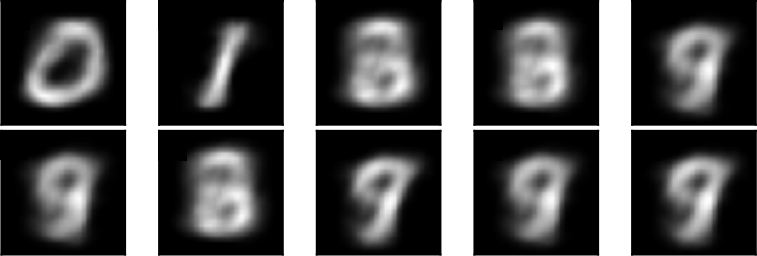
\includegraphics[width=\textwidth]{observational/img/vae/vae_AVG_ls1.png}
         \caption{Latent size $=1$}
     \end{subfigure}
     \hfill
     \begin{subfigure}[b]{0.47\textwidth}
         \centering
         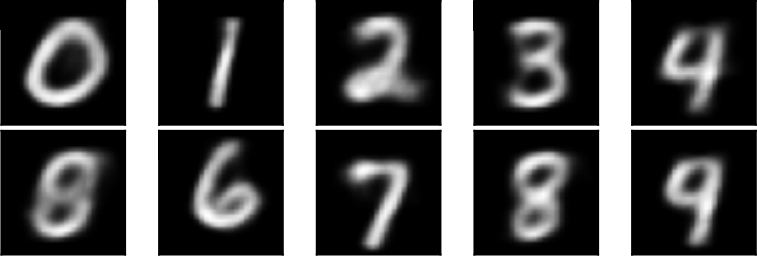
\includegraphics[width=\textwidth]{observational/img/vae/vae_AVG_ls5.png}
         \caption{Latent size $=5$}
     \end{subfigure} 
     \par\bigskip
     \begin{subfigure}[b]{0.47\textwidth}
         \centering
         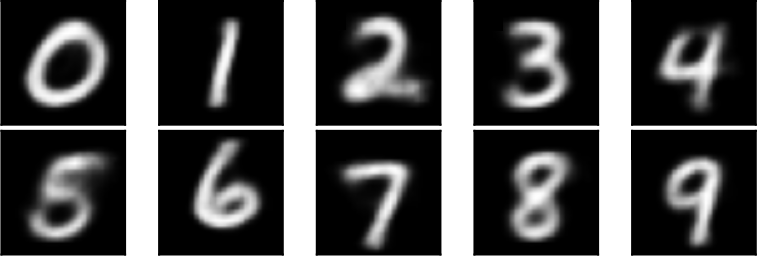
\includegraphics[width=\textwidth]{observational/img/vae/vae_AVG_ls9.png}
         \caption{Latent size $=9$}
     \end{subfigure} 
     \hfill
     \begin{subfigure}[b]{0.47\textwidth}
         \centering
         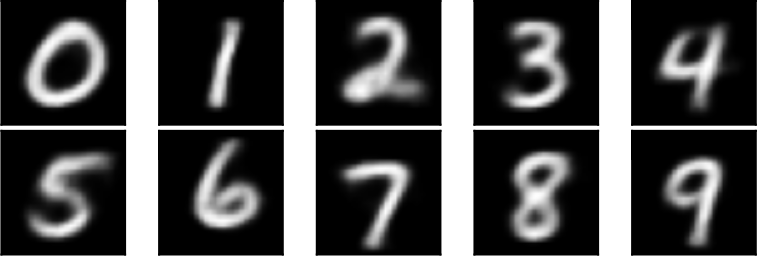
\includegraphics[width=\textwidth]{observational/img/vae/vae_AVG_ls10.png}
         \caption{Latent size $=10$}
     \end{subfigure}
     \par\bigskip
     \begin{subfigure}[b]{0.47\textwidth}
         \centering
         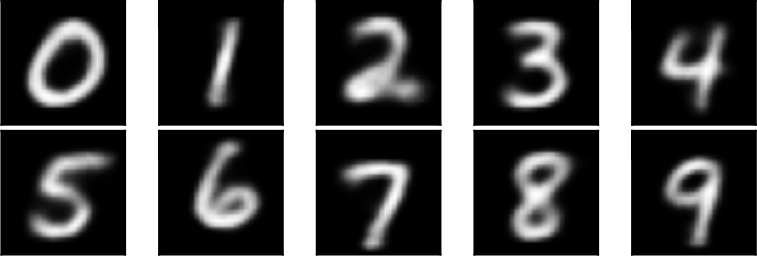
\includegraphics[width=\textwidth]{observational/img/vae/vae_AVG_ls20.png}
         \caption{Latent size $=20$}
     \end{subfigure} 
     \hfill
     \begin{subfigure}[b]{0.47\textwidth}
         \centering
         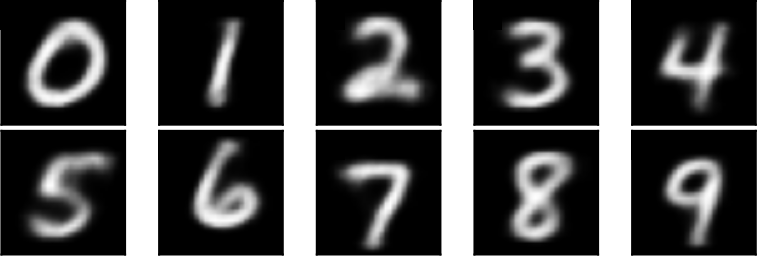
\includegraphics[width=\textwidth]{observational/img/vae/vae_AVG_ls50.png}
         \caption{Latent size $=50$}
     \end{subfigure}
     \caption[Latent size influence on VAE average input reconstruction]{Latent size influence on Variational Autoencoder average input reconstruction.}
    \label{fig:vae-latent-recon}
\end{figure}
